% chapters/09-growth-scaling.tex

\chapter{Growth and Scaling Strategies}\label{ch:growth-and-scaling-strategies}

I remember Sarah, the fintech founder we met earlier.\ She had successfully launched her payment solution, gaining steady traction in her initial market segment.\ ``Dele,'' she said, stirring her drink thoughtfully, ``we've got the foundation right. But how do we really scale this thing?''

That question --- how to scale effectively in Nigeria --- is one I've heard countless times, in different accents, from entrepreneurs across various sectors. The answer, I've learned, isn't just about having the right strategy on paper. It's about understanding what I call the ``Nigerian Scale Dance'' --- the delicate balance between ambition and reality, between speed and sustainability.

\begin{importantbox}
When Sarah returned much later, her business had increased in size --- not because she followed some generic growth playbook, but because she'd learned to dance to Nigeria's unique rhythm. This chapter will show you how to master that same dance.
\end{importantbox}

\section{The Scale-Smart Framework}\label{sec:scale-smart-framework}

Let me share something I learned while scaling Firmbird: In Nigeria, scaling isn't just about getting bigger --- it's about getting smarter. Here's what I call the ``Scale-Smart Matrix'':

\begin{tcolorbox}[colback=white,colframe=primarydark,title=\textbf{Scale-Smart Components}]
\begin{itemize}
    \item \textbf{Systems}
    Build processes that can handle 10x your current volume

    \item \textbf{Market}
    Understand which segments are ready for expansion

    \item \textbf{Assets}
    Invest in scalable resources and relationships

    \item \textbf{Risk}
    Maintain control as you accelerate growth

    \item \textbf{Team}
    Develop leadership that can drive sustainable expansion
\end{itemize}
\end{tcolorbox}

Remember Mike, our e-commerce entrepreneur from Chapter 3? His first attempt at scaling nearly broke his business. ``I thought scaling meant doing everything bigger,'' he told me later. ``I learned it actually means doing everything better.''

\section{Regional Growth Pathways}\label{sec:regional-growth-pathways}

Each region brings its own growth DNA to Nigeria. Let's explore how to leverage these unique strengths:

\subsection{UK Financial Services Evolution}\label{subsec:uk-financial-evolution}

Sarah's journey offers valuable lessons here. She scaled her fintech operation using what I call the ``Trust-Growth Spiral'':

\begin{tcolorbox}[colback=white,colframe=primary,title=\textbf{Financial Services Growth Model}]
\begin{enumerate}
    \item \textbf{Regulatory Capital Growth}
    \begin{itemize}
        \item Start with minimum requirements
        \item Build reserves systematically
        \item Expand licensing gradually
    \end{itemize}

    \item \textbf{Product Portfolio Expansion}
    \begin{itemize}
        \item Begin with core services
        \item Add complementary products
        \item Integrate new technologies
    \end{itemize}

    \item \textbf{Market Segment Penetration}
    \begin{itemize}
        \item Focus on initial niche
        \item Expand to adjacent segments
        \item Scale across sectors
    \end{itemize}
\end{enumerate}
\end{tcolorbox}

``The key,'' Sarah shared during a webinar, ``was realizing that in Nigerian financial services, trust scales faster than technology.''

\subsection{US Tech Platform Scaling}\label{subsec:us-tech-scaling}

Remember Mike's e-commerce platform? After his initial scaling challenges, we developed what I now call the ``Nigerian Tech Scaling Triangle'':

\begin{figure}[h]
    \centering
    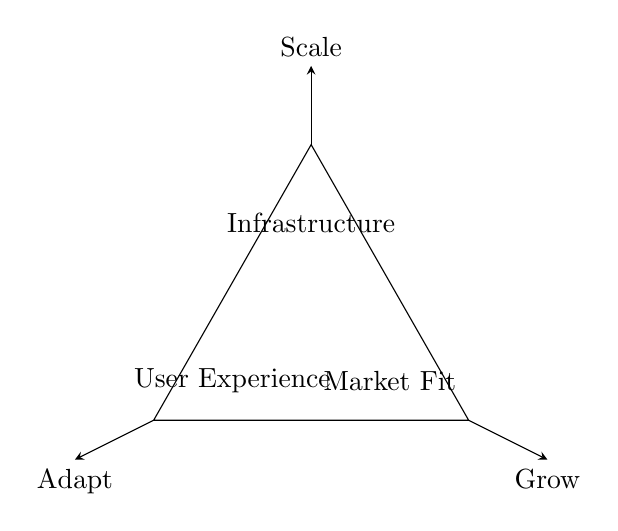
\begin{tikzpicture}
        % Tech Scaling Triangle visualization
        \draw (0,0) -- (4,0) -- (2,3.5) -- cycle;
        \node at (2,2.5) {Infrastructure};
        \node at (1,0.5) {User Experience};
        \node at (3,0.5) {Market Fit};

        % Add scaling indicators
        \draw[-stealth] (2,3.5) -- (2,4.5) node[above] {Scale};
        \draw[-stealth] (0,0) -- (-1,-0.5) node[below] {Adapt};
        \draw[-stealth] (4,0) -- (5,-0.5) node[below] {Grow};
    \end{tikzpicture}
    \caption{Tech Scaling Triangle}
    \label{fig:tech-triangle}
\end{figure}

\subsection{UAE Trade Network Development}\label{subsec:uae-trade-development}

Ahmed's trading operation provides an excellent case study in scaling trade networks. His approach, which I call the ``Hub-and-Spoke Plus'' model, revolutionized how he scaled his import/export business:

\begin{tcolorbox}[colback=white,colframe=primarydark,title=\textbf{Trade Network Scaling}]
\begin{itemize}
    \item \textbf{Core Hubs}
    \begin{itemize}
        \item Lagos Central Hub
        \item Regional Distribution Centers
        \item International Connection Points
    \end{itemize}

    \item \textbf{Network Spokes}
    \begin{itemize}
        \item Local Partner Network
        \item Transport Corridors
        \item Market Access Points
    \end{itemize}

    \item \textbf{The "Plus" Elements}
    \begin{itemize}
        \item Digital Integration
        \item Payment Networks
        \item Compliance Systems
    \end{itemize}
\end{itemize}
\end{tcolorbox}

``In Nigeria,'' Ahmed told members on , ``your network is your net worth. But scaling that network requires systematic thinking.''

\subsection{Canadian Sector Innovation}\label{subsec:canadian-sector-innovation}

Lisa's AgriTech venture scaled through what I now call the ``Innovation Multiplication Model'':

\begin{center}
\begin{tabularx}{\textwidth}{>{\raggedright\arraybackslash}X >{\centering\arraybackslash}X >{\raggedright\arraybackslash}X}
    \toprule
    \textbf{Phase} & \textbf{Focus} & \textbf{Outcome} \\
    \midrule
    Foundation & Core Technology & Market Validation \\
    Expansion & Partner Network & Regional Growth \\
    Scaling & Integration & National Presence \\
    Optimization & Efficiency & Market Leadership \\
    \bottomrule
\end{tabularx}
\end{center}

\section{The Growth Readiness Framework}\label{sec:growth-readiness}

Before you start scaling, run through what I call the ``Ready-Set-Grow'' checklist:

\begin{tcolorbox}[colback=white,colframe=primarydark,title=\textbf{Growth Readiness Assessment}]
\begin{enumerate}
    \item \textbf{Ready: Foundation Check}
    \begin{itemize}
        \item Core operations stable
        \item Basic metrics positive
        \item Initial team solid
        \item Customer base established
    \end{itemize}

    \item \textbf{Set: Scale Preparation}
    \begin{itemize}
        \item Systems documented
        \item Resources allocated
        \item Team aligned
        \item Market mapped
    \end{itemize}

    \item \textbf{Grow: Execution Planning}
    \begin{itemize}
        \item Growth targets set
        \item Resources ready
        \item Timeline established
        \item Metrics defined
    \end{itemize}
\end{enumerate}
\end{tcolorbox}

\section{Scaling Pitfalls}\label{sec:scaling-pitfalls}

Let me share what I call the ``Four Fatal Flaws'' of scaling in Nigeria:

\begin{enumerate}
    \item \textbf{The Speed Trap}
    I watched a talented US entrepreneur crash and burn because he scaled too fast. ``I thought I could grow at Silicon Valley speed in Lagos,'' he told me afterward. The lesson? Pace your growth to match market realities.

    \item \textbf{The Copy-Paste Problem}
    A fintech founder tried to replicate their London growth strategy in Nigeria. Three months and significant losses later, they learned that Nigerian scaling requires Nigerian solutions.

    \item \textbf{The Resource Race}
    ``We'll just throw money at it,'' a confident investor told me. Six months later, he understood that in Nigeria, smart resources beat big resources every time.

    \item \textbf{The Control Crisis}
    An AgriTech founder lost control of her operation trying to scale too many segments simultaneously. ``Focus and phase,'' became her mantra after we helped her reorganize.
\end{enumerate}

\section{Quality Control in Growth}\label{sec:quality-growth-control}

One of my favorite Nigerian proverbs says, ``A child who walks carefully can travel a hundred roads.'' This wisdom applies perfectly to scaling. Here's my ``Quality-Scale Matrix'':

\begin{center}
\begin{tabularx}{\textwidth}{>{\raggedright\arraybackslash}X >{\centering\arraybackslash}X >{\raggedright\arraybackslash}X}
    \toprule
    \textbf{Growth Area} & \textbf{Quality Metrics} & \textbf{Control Methods} \\
    \midrule
    Operations & Performance KPIs & Regular Audits \\
    Customer Service & Satisfaction Rates & Feedback Systems \\
    Product Delivery & Quality Standards & Testing Protocols \\
    Team Performance & Productivity Metrics & Training Programs \\
    \bottomrule
\end{tabularx}
\end{center}

\section{Sustainable Growth Planning}\label{sec:sustainable-growth}

Remember Lisa's AgriTech venture? Her sustainable growth came from what I call the ``Triple-Bottom-Line Scale'':

\begin{tcolorbox}[colback=white,colframe=primarydark,title=\textbf{Sustainable Scaling Components}]
\begin{itemize}
    \item \textbf{Economic Sustainability}
    \begin{itemize}
        \item Revenue growth targets
        \item Cost optimization plans
        \item Investment strategies
        \item Profit sustainability
    \end{itemize}

    \item \textbf{Social Impact}
    \begin{itemize}
        \item Community development
        \item Job creation metrics
        \item Skills development
        \item Local partnership growth
    \end{itemize}

    \item \textbf{Environmental Responsibility}
    \begin{itemize}
        \item Resource efficiency
        \item Waste reduction
        \item Green technology adoption
        \item Environmental compliance
    \end{itemize}
\end{itemize}
\end{tcolorbox}

\section{Your Growth Action Plan}\label{sec:growth-action-plan}

Let's turn these insights into action. Here's your growth planning workshop:

\begin{workshopbox}
\textbf{Growth Strategy Development}

1. Assessment Phase
\begin{itemize}
    \item Current state analysis: \_\_\_\_\_\_\_\_\_
    \item Growth readiness score: \_\_\_\_\_\_\_\_\_
    \item Resource inventory: \_\_\_\_\_\_\_\_\_
\end{itemize}

2. Strategy Development
\begin{itemize}
    \item Growth model selection: \_\_\_\_\_\_\_\_\_
    \item Timeline planning: \_\_\_\_\_\_\_\_\_
    \item Resource allocation: \_\_\_\_\_\_\_\_\_
\end{itemize}

3. Implementation Planning
\begin{itemize}
    \item First 90 days: \_\_\_\_\_\_\_\_\_
    \item Key milestones: \_\_\_\_\_\_\_\_\_
    \item Success metrics: \_\_\_\_\_\_\_\_\_
\end{itemize}
\end{workshopbox}

\begin{communitybox}
Connect with fellow entrepreneurs and access additional resources on the Africa Growth Circle:
\begin{itemize}
    \item Detailed growth planning templates
    \item Expert scaling workshops
    \item Peer learning sessions
    \item Regional networking events
    \item Monthly scaling masterclasses
\end{itemize}
Visit circle.counseal.com to join the conversation.
\end{communitybox}

\begin{importantbox}
Remember, in Nigeria, sustainable scaling isn't about how fast you can grow --- it's about how well you can grow. In our final chapter, we'll explore how to future-proof your business for long-term success in the Nigerian market.
\end{importantbox}